\documentclass{article}

% Language setting
% Replace `english' with e.g. `spanish' to change the document language
\usepackage[english]{babel}

% Set page size and margins
% Replace `letterpaper' with`a4paper' for UK/EU standard size
\usepackage[letterpaper,top=2cm,bottom=2cm,left=3cm,right=3cm,marginparwidth=1.75cm]{geometry}

% Useful packages
\usepackage{amsmath}
\usepackage{graphicx}
\usepackage{natbib}
\bibliographystyle{apalike}
\usepackage{float}
\graphicspath{ {./figures/} }
\usepackage[colorlinks=true, allcolors=blue]{hyperref}
\usepackage{csquotes}
\MakeOuterQuote{"}
\title{Don't Use Dinos (DUD): Final Report}
\author{Israel Bonilla, Nick Jadallah, Mike Lau, \\
Grace Sommers, Jackson Swilley, and Hannah Williams}

\begin{document}
\maketitle
\section*{Background}
\subsection*{Scientific Motivation}
As anthropogenic climate change prompts the global community to reduce greenhouse gas (GHG) emissions, aviation has emerged as particularly difficult to decarbonise. Continuing aviation at scale is important to the achievement of the UN’s Sustainable Development Goals (SDGs), as the sector contributes significantly to hunger reduction (SDG 2) through airlifted food, and to decent work and economic growth (SDG 8) through the creation of 87.7 million jobs and \$3.5 trillion in economic activity \citep{air_transport_action_group_sustainable_2020}. Yet, its decarbonisation faces significant challenges, both regulatory, due to its international nature, and technical, as the strict requirements of flight narrow alternatives to fossil-fuels.\par
Aviation emissions currently primarily come from the combustion of Jet A-1 fuel. To forecast how the international aviation sector might reduce emissions while continuing to deliver societal benefit, pathways have been developed by government \citep{department_for_transport_jet_2021,itf_decarbonising_2021}, climate groups \citep{climate_change_committee_sixth_2020, transport__environment_roadmap_2018, fleming_flight_2020}, and industry stakeholders \citep{sustainable_aviation_sustainable_2020, nlr_-_royal_netherlands_aerospace_centre_destination_2021}. In addition to demand reduction and improved fuel efficiency, these pathways project that Sustainable Aviation Fuels (SAFs) and liquid hydrogen (LH2) will provide most in-sector emissions reductions for international flight, with negative emissions technologies (NETs) offsetting remaining emissions. SAFs offer identical or improved characteristics to Jet A-1 with reduced life-cycle carbon, but often require millions of hectares of land, millions of tonnes of water, and terawatt-hours of energy to fuel significant portions of flight volume. Hydrogen could offer zero point-of-consumption emissions with reduced resource requirements, but aviation technologies cannot currently accommodate it. \par
From a regulatory perspective, the International Civil Aviation Organization’s (ICAO) Carbon Offsetting and Reduction Scheme for International Aviation (CORSIA) is the current international standard for aviation decarbonisation, but it does not require emissions reductions. Under CORSIA, airlines will only be required to offset growth in carbon emissions on international routes beyond 2020 levels after 2027, and can volunteer to offset these emissions from 2021-2026, relying on NETs to allow growth in flight volume with constant emissions \citep{icao_2_2021}. \par
Sustainable development is often defined through reference to the Brundtland report (\citeyear{keeble_brundtland_1988}), which pushed meeting “the needs of the present without compromising the ability of future generations to meet their own needs,” or to balancing the “triple bottom line” of societal, economic, and environmental interests \citep{elkington_towards_1994}. On a global scale, environmental sustainability is often considered in relation to living within planetary limits \citep{lin_ecological_2018,meadows_limits_2004}. Though climate change is among the most immediate of these limits, exceeding and degrading earth’s biocapacity through multi-sectoral overuse of land, water, and energy resources would lead to substantial environmental and societal damages. \par
Though aviation is economically beneficial, its current emissions endanger its societal and economic benefits. However, in decarbonising (SDG 13), the implementation of low-carbon, but high environmental footprint, technical options will coincide with projected jumps in flight volume to significantly increase the land, water, and energy footprints associated with aviation, leading to potential conflicts between decarbonisation and other SDGs, like Life on Land (SDG 14) or Clean Water and Sanitation (SDG 6). As work from the Potsdam Institute for Climate Impact Research (PIK) and the Global Footprint Network has highlighted, humanity’s current overshoot of global resource limits is unsustainable; indicating that development and decarbonising transitions must minimize expansions of resource use \citep{holmatov_land_2019}.\par
Current aviation decarbonisation pathways, though more ambitious than CORSIA, focus primarily upon emissions reductions and its associated co-benefits while abstracting away environmental footprint concerns. The recent Jet Zero strategy consultation released by the United Kingdom’s (UK) Department for Transport, for instance, dedicates two paragraphs to the sustainable sourcing of fuels upon which it pins significant emissions reductions \citep[27]{department_for_transport_jet_2021}. Destination 2050, a pathway to net-zero aviation for the European Union (EU) released by aviation industry bodies, dedicates four pages to the emissions associated with land use change from Sustainable Aviation Fuels (SAFs), and includes little on minimizing or quantifying resource use \citep{nlr_-_royal_netherlands_aerospace_centre_destination_2021}. In planning the ICAO’s long-term ambitions, the ICAO has explored SAFs, carrying out a benchmarking process for induced land use change (ILUC) emissions but offering little analysis of resource consumption \citep{international_civil_aviation_organisation_icao_corsia_2019}.\par 
As indicated by the many recent pathways towards decarbonization, the aviation sector is planning its climate-friendly transition. Thus, an opportunity exists to integrate environmental footprint into the industry’s choices as it moves towards climatic sustainability. With a plethora of emissions-reductions scenarios plausible for the aviation industry, understanding the resource footprints associated with net zero flight systems is key to discovering most-sustainable paths. \par

\subsection*{Existing Work}
\paragraph{} An environmental footprint model for multiple AAF production pathways was developed, contributing a means of quickly evaluating the land, water, and energy use, annual emissions recaptured, and capital resource requirements associated with various aviation decarbonisation scenarios. This model can be used to quantify the environmental costs associated with different policies, technologies, and support mechanisms. Based upon the novel inclusion of feedbacks related to land, energy, water, and direct air carbon capture (DACC), new estimations were made of the environmental footprints of several fuel production pathways. However, the existing model had some significant limitations. First, it was difficult to interact with and change, as it was one long MatLab script. This, combined with the large number of constants, inconsistent unit choice, and some WET code made the previous version difficult to read or manipulate meaningfully without immense effort. Second, the existing code had little flexibility or separation of concerns. Everything was in one file, with many different subsections of code pipelining one into the next. It was impossible to make independent changes to portions of the file. This was a major limitation in that new fuel production methods, new feedstocks, new feedback mechanisms, and new data could not be input, limiting the code to reproducing variations of the outputs already gathered. Furthermore, the existing feedback accounting system was meaningfully limited. As the current iteration ignored several cycling dynamics and implemented feedbacks primarily through certain one-directional relationships and a single feedback loop representing DACC, it was not nearly representative of real-world dynamics. 

\section*{Project Goals}
Our development team set out the following goals to address the challenges outlined in the Scientific Motivation and to improve the existing environmental footprint model. Overall, we aimed to create a new modular environmental footprint model and maintaining it on the version control site GitHub. Specifically, the model was transcribed from MATLAB, the language in which it was originally written, to Python. Object-oriented programming approaches were to be employed to create a software that is modular and more suited for future development. The team also aimed to create a suite of tests to check the functionality of features. Finally, we wanted to generate clear and current documentation in an automated fashion to encourage collaboration and development of additional features. We successfully completed several of these goals - a much improved, object-oriented version of the previous code has been maintained on GitHub, testing is automatically carried out on each push to the repository, and documentation can be generated upon request. However, we were not entirely successful in our goals, as will be discussed in \textbf{Development Process}. 


\section*{System Design}
The core element of the system in code is the \texttt{Agent} abstract base class (ABC), with the main idea being that every process, fuel, and feedstock is responsible for some environmental footprint, which itself exists as a class central to the inner workings of the design. Every concrete class therefore owns a footprint. The idea is to then create each of the fuels via each of the processes according to the specification of the user, with the user specifying the proportions of each fuel type. 

The \texttt{Footprint} class, implemented using the \texttt{@dataclass} decorator in Python, has seven core attributes, all of type double: \texttt{land}, the land footprint in hectares; \texttt{CO2\_emm}, the CO2 emissions in kg; \texttt{CO2\_used}, kg CO2 consumed that does not need to be recaptured; \texttt{blue}, the blue water footprint in kg; \texttt{green}, the green water footprint, which does not participate in feedback; \texttt{electric}, the electricity consumption in MJ; \texttt{nat\_gas}, the natural gas footprint in kg; and \texttt{capex}, the capital expenditure in English pounds. Packaging these attributes into a single class not only signals their logical coherence but is also conducive to the implementation of "Footprint algebra": the aggregation of footprints for the different processes, fuels, and feedstocks which combine into one total footprint. The default for each of these seven attributes is 0 in the \texttt{Footprint} constructor, so an \texttt{Agent} with, say, no capital cost can instantiate its footprint without even needing to know that \texttt{capex} is an attribute of \texttt{Footprint}.

The complete UML diagram is shown in Fig.~\ref{fig:UML} and described in more detail below.

\begin{figure}[H]
    \centering
    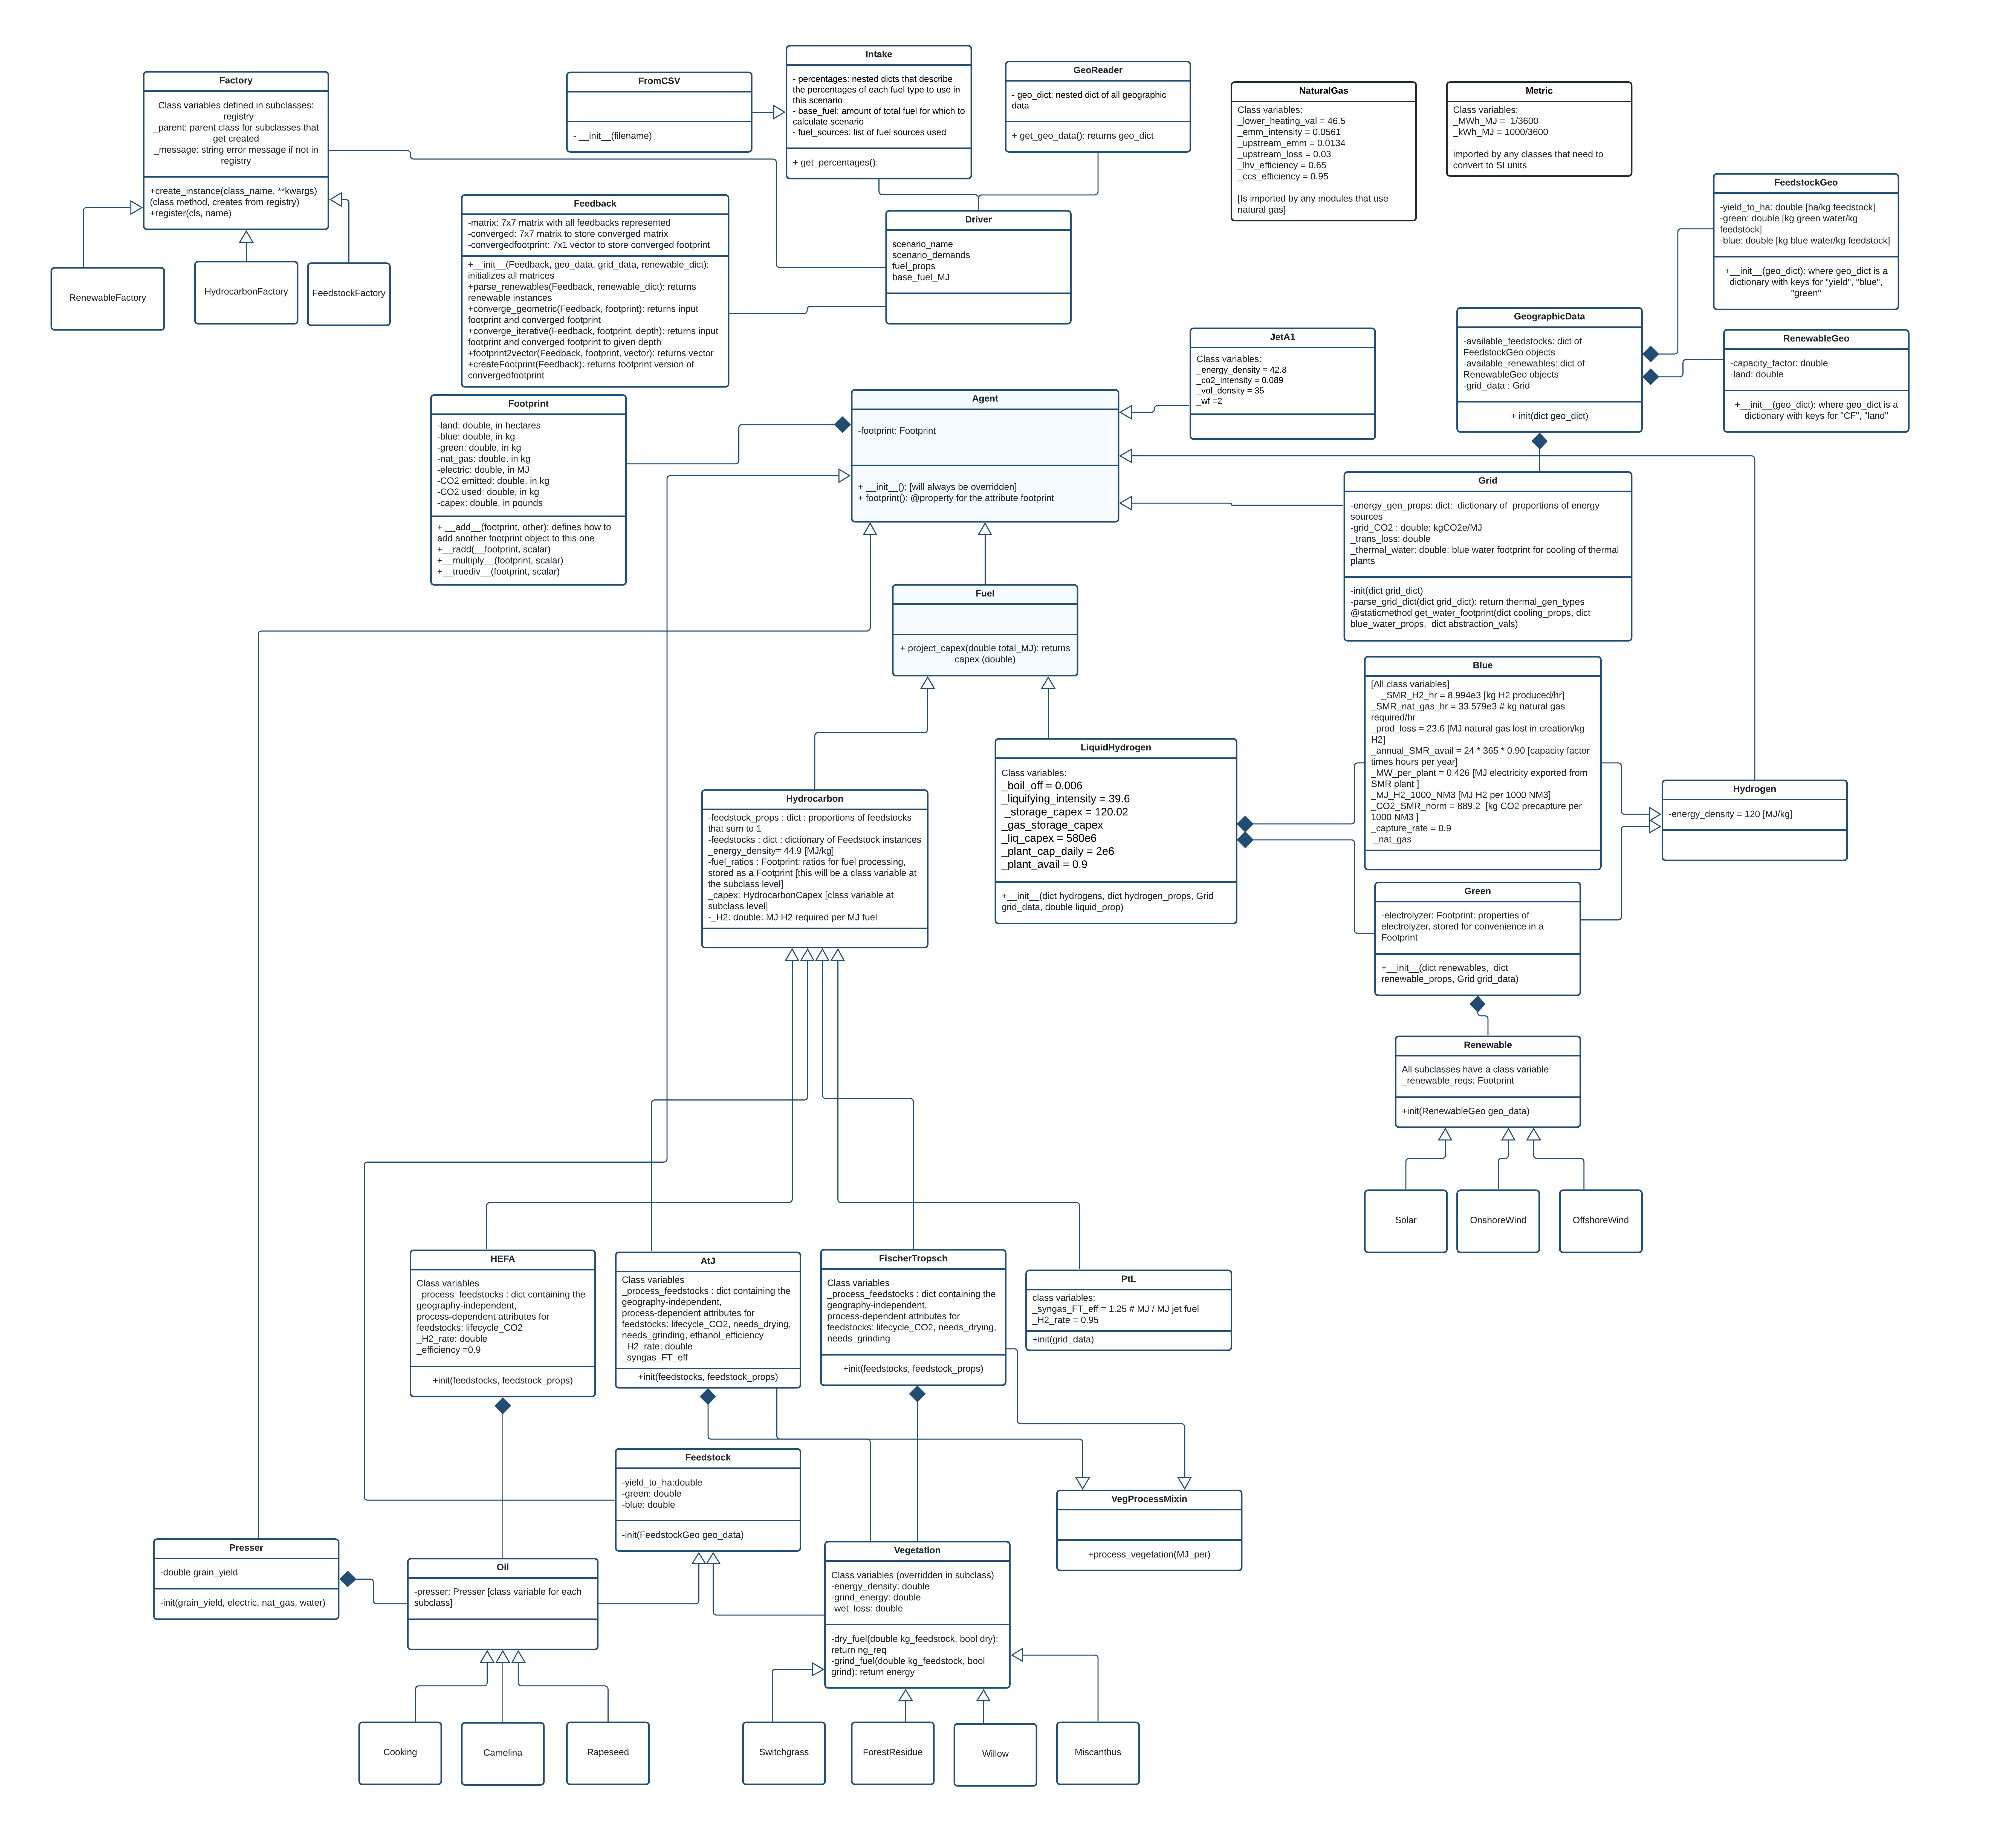
\includegraphics[width=1\textwidth]{figures/UML 3.0.jpeg}
    \caption{UML Class Diagram}
    \label{fig:UML}
\end{figure}

\subsection*{Subclasses of \texttt{Agent}}
Subclasses of \texttt{Agent} fall into several different categories. All of them construct a \texttt{Footprint} on a per-unit basis; that is, every instance of \texttt{Renewable} and \texttt{Fuel} computes its footprint per MJ of fuel, while it is more natural for instances of \texttt{Feedstock} and \texttt{Presser} to compute footprints per kg. Then, to determine footprint for a total demand of fuel in MJ, we simply take the weighted sum over the main Agents, given user input for the proportion of each fuel type used. These main fuels are instances of the abstract base class \texttt{Fuel}, which directly inherits from \texttt{Agent}. \texttt{Fuel} requires that its concrete subclasses, in addition to producing a \texttt{Footprint}, also implement the method \texttt{project\_capex(total\_MJ)}. This is because, while the individual raw materials comprising the fuels (e.g., the feedstocks and renewable energy sources) can compute their capital expenditure on a per-unit basis, instances of the \texttt{Fuel} subclasses \texttt{Hydrocarbon} and \texttt{LiquidHydrogen} have an additional capital expenditure that depends on the total number of power plants used. The number of power plants varies with the total amount of fuel in a stepwise manner.

Aside from jet fuel, all fuels are instances of either \texttt{Hydrocarbon} or \texttt{LiquidHydrogen}. The \texttt{Hydrocarbon} branch of the class diagram has a high degree of structure, and benefited greatly from the use of the factory design pattern. First, we use \texttt{HydrocarbonFactory} to instantiate concrete subclasses of \texttt{Hydrocarbon}, which are decorated to self-register, making it easy to implement additional subclasses in the future. At present four subclasses are implemented, and with the exception of \texttt{PtL}, a strange hydrogen-hydrocarbon hybrid, they all synthesize feedstocks such as vegetation or plant-based oils in user-specified proportions. Hence, each of these subclasses is instantiated with a dictionary of instances of the class \texttt{Feedstock}, which are instantiated in the driver prior to instantiating the \texttt{Hydrocarbon} objects.  \texttt{Feedstock} has two subclasses, \texttt{Oil} (which is used by \texttt{HEFA}) and \texttt{Vegetation} (which is used by \texttt{FischerTropsch} and \texttt{AtJ}), both of which in turn have concrete subclasses that differ with respect to certain innate biological/physical attributes and are instantiated using the \texttt{FeedstockFactory}. Crucially, all instances of \texttt{Feedstock}, as well instances of \texttt{Presser} (which are class variables of all \texttt{Oil} subclasses) are themselves subclasses of \texttt{Agent}. As such, they are responsible for computing a footprint that depends only on the inherent properties of the feedstock, \textit{not} the process that uses them. This means that \texttt{FischerTropsch} and \texttt{AtJ}, which use many of the same vegetation feedstocks, can be instantiated with the same dictionary of feedstocks but process them slightly differently. To adhere to the DRY coding paradigm, we have these classes inherit from the mixin class, \texttt{VegProcessMixin}, which incorporates the footprints of the constituent vegetation feedstocks into the footprints of the fuels that process them.

Meanwhile, the relatively simple structure on the \texttt{LiquidHydrogen} cloaks a rather complex interplay of physical processes. \texttt{LiquidHydrogen} can be thought of as using \texttt{Hydrogen} as its "feedstock" (although \texttt{Hydrogen} itself is not a subclass of \texttt{Feedstock} since it differs substantially in terms of attributes). Analogously to how we separated out the inherent footprints of individual \texttt{Feedstock} objects from the additional footprints for processing them in \texttt{Hydrocarbon}, here we sought to disentangle the footprint of "raw" hydrogen (i.e., without liquefaction) from the footprint for the liquefaction process. The ABC \texttt{Hydrogen} has two subclasses, \texttt{BlueHydrogen} (which takes no inputs and has only class variables) and \texttt{GreenHydrogen}. The latter takes a dictionary of \texttt{Renewable} objects, themselves instantiated via the \texttt{RenewableFactory}, and combines their aggregated footprints with its own footprint for the electrolysis process.

A complicating feature of \texttt{LiquidHydrogen} is that most of the \texttt{Hydrocarbon} fuels also use hydrogen, but without the need for liquefaction. Therefore, after some false starts, we found it simplest to implement this interplay between hydrocarbons and hydrogens by having each instance of \texttt{Hydrocarbon} carry around an attribute \texttt{H2} in addition to a footprint, defined as the amount of hydrogen, in MJ, required in the creation of 1 MJ of hydrocarbon fuel. In the driver, \texttt{LiquidHydrogen} is instantiated \textit{after} all the hydrocarbons, and included in its constructor is a parameter, \texttt{liquid\_prop}, that specifies the proportion of hydrogen that needs to be liquefied. This allows us \texttt{LiquidHydrogen} to calculate, on a per-MJ basis, the footprint for \textit{all} hydrogen needed in a given scenario.

\subsection*{Incorporating Geographic Data}
One of the major challenges of this project was the incorporation of geographically specific data in a separable and modular fashion. In our design, we accomplished this through the combination of several classes, specifically \texttt{geo\_reader}, \texttt{geographic\_data}, and \texttt{Grid}. The user of the code was expected to input a nested dict of dicts, each of which held some geographic data labelled with its general use, as is discussed in the \textbf{User Input} section. These were read in through \texttt{geo\_reader}, and could then be used to instantiate \texttt{Agent}s throughout the code with geographic specificity. This solution allowed for all required geographically specific data to be relatively easily accessed and used by \texttt{Agent}s.  

\subsection*{Implementation of \texttt{Feedback}}
The final section of the code, \texttt{Feedback}, is functionally implemented as a relatively simple footprint modifier, yet due to the multi-sectoral nature of the physical processes it represents, the inputs for \texttt{Feedback} stretch from \texttt{geo\_data} to dicts of instances of \texttt{Renewables}, to entire \texttt{Grid} objects. Inputs from each of these disparate parts of the UML are required to build the fundamental attribute of the \texttt{Feedback} object - the feedback matrix. Once instantiated with these various data, \texttt{Feedback} can take any footprint generated by the rest of the instantiated \texttt{Agent}s and calculate a new footprint including systemic feedbacks, returning both the converged footprint and the original footprint. This allows for flexibility in terms of output results. Considering potential stakeholders in this project, some, such as fuel manufacturers, may only be interested in the per-MJ footprint of their fuels and as such may want to consider system convergence on one unit of one fuel, whereas others, regulatory stakeholders for instance, may wish to consider the footprint of an entire system architecture. The particular structure of \texttt{Feedback} allows for both use-cases to be fulfilled. In class inheritance terms, \texttt{Feedback} is relatively simple, since it is used neither as a feedstock nor process for any other agent. As such, it is functionally an \textit{ex-post-facto} calculation that may be applied to any given footprint.

\subsection*{User Input}
One of the main goals of this project was extending the original thesis to be agnostic to geography, specifically that the code will run provided it receives sufficient information about a target airport cluster. In conjunction with the user-supplied proportions of each fuel, the program needed to take in much more information than could reasonably be supplied by command-line arguments. Therefore, we elected to use a pair of CSV files to serve this purpose. \par

\begin{figure}[H]
    \centering
    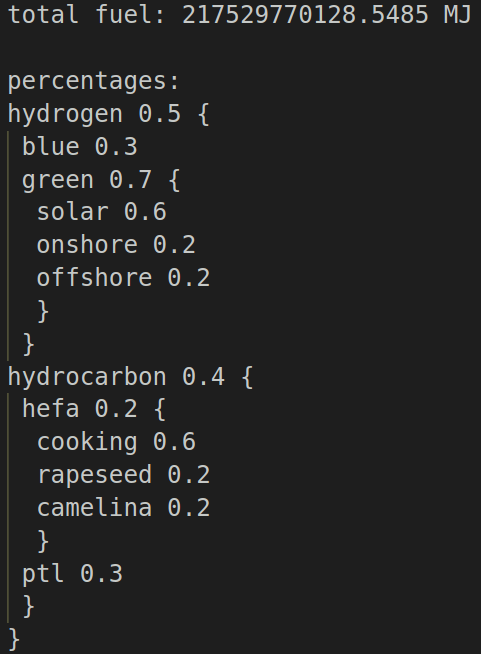
\includegraphics[scale=0.3]{figures/sample_prop_csv.png}
    \caption{Sample Proportion Input CSV}
    \label{fig:Sample Proportion CSV}
\end{figure}
For user input of fuel proportions, we specify a total fuel requirement in MJ at the top, which will depend upon which airport cluster the user cares about. Then, the file delves into percentages, where the user must specify proportions of the first subgroups, Hydrogens and Hydrocarbons. Then, for each subtype of those fuels, the user must specify the required proportions of subtypes of fuels, so on and so forth until the full depth of fuel types is reached, resulting in a file similar to the above sample.

\begin{figure}[H]
    \centering
    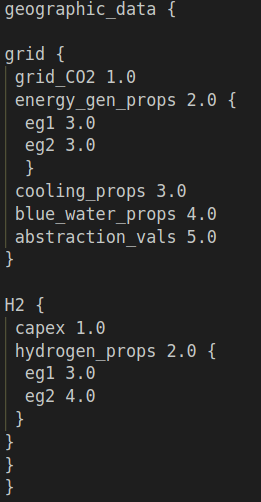
\includegraphics[scale=0.4]{figures/sample_geo.png}
    \caption{Sample Geographic Data CSV}
    \label{fig:Sample Proportion CSV}
\end{figure}

Similarly to the proportion CSV, the geo-data CSV specifies a name and then a value for geographically dependent constants. For constants with constituent proportions, the depth and values of these are specified in the same way, just like the above sample.

\section*{Development Process}
A major challenge of this project was the class design. We found it difficult to distill the real-world scenario we were trying to capture, which entails hundreds of constants, into a simple class hierarchy.

With the resident expert of the group felled by illness, the rest of us forged ahead in trying to make sense of the 1500+ lines of MatLab code bestowed upon us. This naturally resulted in a series of false starts. We began by tackling the sea of constants and mapping out the categories to which they belonged and the relationships between them. In an attempt not to fall too far behind, we felt compelled to start the actual coding phase of the project, but with an admittedly hazy sense of how the different parts of the system interacted, we lacked a solid plan for how to express the footprint produced by each fuel. In our first iteration, each subclass of \texttt{Hydrocarbon} just implemented a method that returned a dictionary \texttt{fuel\_reqs}, with key-value pairs corresponding to different aspects of the footprint (e.g. carbon emissions, blue water, etc.). While an improvement upon the MatLab code, in which each of these aspects of the footprints were held in different variable with no logical coherence, this pinned us to a specific implementation (a dictionary) and was not conducive to conglomerating the footprints of different fuels (for which the keys in \texttt{fuel\_reqs} could vary).  Only after an extensive discussion with Gabe did we come to realize that this dictionary should instead be a full-fledged class, \texttt{Footprint}, and that nearly everything is a footprint maker (inheriting from the abstract base class \texttt{Agent}). This provided a layer of abstraction when manipulating footprints. For example, an early version of the class \texttt{FischerTropsch} was tightly coupled to the \texttt{Vegetation} class, to which the individual feedstocks fed into the process belong. Once we developed the \texttt{Footprint} class with its attendant "footprint algebra" and separated out the inherent attributes of the feedstocks from their process-specific properties, this code simplified greatly.

Although settling upon the basic structure of footprints and agents resolved some of our programming challenges, we still faced difficulties on the scientific side which hindered progress on the coding side. In particular, our understanding of what things were true constants (which later became class variables) vs. parameters that depend on the geography but remain static during the lifetime of the code was continually shifting. As such, the \texttt{GeographicData} class became an amorphous black box whose attributes were not pinned down until late in the development stage. Despite our efforts to write robust, modular code, the shifting goalposts inevitably affected not just the \texttt{GeographicData} class itself but also the constructors and attributes for the classes that were expected to "eat" geographic data - a substantial portion of our code. This in turn entailed repeated revisions to the testing code, since objects that at first were expected to be instantiated with some geographic parameters were later found not to depend on geography, or vice versa. Making the attributes of \texttt{GeographicData} instances of a series of small classes (\texttt{FeedstockGeo}, \texttt{RenewableGeo}, and \texttt{HydrocarbonGeo}, the last of which became obsolete once we realized its attributes were true constants) mitigated this problem somewhat, since if we later found that \texttt{Renewable} objects would need to be instantiated with another geographic parameter, we could just add that to the \texttt{RenewableGeo} class with minimal modifications to \texttt{Renewable} itself.

Handling constants proved to be an immense task. For each of the $\approx$400 constants, we had to decide whether to include them in \texttt{geographic\_data}, or to include them in class attributes, if they were deemed non-geographically dependent. Collating and reading in each of these constants, combined with unit conversion and normalization took far longer than expected, and was one of the major hurdles to the profiling of this project. 

The last part of the code to come together was the implementation of the feedback, including the direct air carbon capture (DACC). After our prior discussions with Gabe, and reconsideration of the set of feedbacks we were looking to represent, a new methodology for computing these feedbacks was devised. We would look to represent them within a matrix, which, we thought, could then be put into a geometric series until it converged, representing the eventual result of our feedback cycles. The convergence of a geometric series of matrices can be represented as seen in equation \ref{eq: Geo_mat}.
\begin{equation}\label{eq: Geo_mat}
\begin{aligned}
    S_n = I + M + M^2 + \cdots + M^{n-1}\\
    \lim_{n\rightarrow\infty} S_n = (I - M)^{-1}
\end{aligned}
\end{equation}
Upon implementation, however, some issues came up with this representation. When computing the converged value of the feedback cycle using equation \ref{eq: Geo_mat}, our converged matrix began showing up with negative values - a clearly wrong result. Our explanation for this phenomenon was that perhaps our feedback cycles were not actually representable as a geometric series, though we were, and still are, confused as to why that may be.

We implemented a second method for calculating the converged feedbacks, which used the non-infinite representation of the geometric series of matrices to calculate feedback to a user-provided depth. This method worked much better than our geometric convergence implementation, providing reasonable values throughout for each depth tested.

We used \texttt{pytest} and Github Actions CI to maintain a consistent testing standard, and to ensure that all of our code would run and give reasonable values. For this project, though, it is worth noting that our tests were primarily verification-based tests: essentially making sure that the output of our implemented code matched the outputs of the previous version of the code to ensure that integrity was maintained. However, there was no effective way to truly validate these results, due to the novel nature of this work and the lack of data from which to validate this model. For some portions of our project where notable changes to the previous code's mathematical foundation were made, such as \texttt{feedback.py}, testing could do even less. As previously calculated values would no longer match, we could only really test for obviously wrong values (i.e. negative or above a certain threshold). These were still able to ensure that the code ran, but validation of correct results was impossible.

Our execution of the Git workflow had mixed success. On the positive side, we only had to deal with a few merge conflicts, which was facilitated by the fact that we were typically working on uncoupled parts of the code. However, since the class design was continually changing, we did not end up using pull requests in the manner we had proposed. Instead, most of the code stayed on various branches with intermittent merges among them, with minimal use of \texttt{dev} and pull requests to \texttt{main} only at the very end. (Figure.)

\section*{Lessons Learned}
Given all the time poured into this project simply for the sake of system design, the most obvious lesson is the necessity of doing due diligence to design before ever writing a piece of code. Had we not followed this adage, the existing code would have had to have been rewritten every single time a design change was made, which was very frequent given the complicated nature of the problem at hand. \par
For those in the group with less exposure to environmental science problems, this was a learning experience in where the mathematical complexity (diesel) lives. This complexity is analogous to the curse of dimensionality in that representing an environmental system requires considering a large number of factors in order to be genuinely reflective of the world at large. 
\par
The entire project was a huge lesson in a variety of software tools, from documentation generation via Sphinx to Continuous Integration on GitHub Actions to general Python best practices. Suffice to say we have all greatly improved as software developers through this project.

\section*{Future Work}

We are most excited about the future development of an optimizer with a user-definable cost function. This tool will allow modelers to prioritize which footprints they are most concerned with and find the combination of fuels, processing methods, and fuel feedstocks that minimizes said footprint. A tool of this magnitude and design could have use cases for city planners, airlines, and environmental scientists. By creating case-specific geographic data objects, this model can be used to explore pathways to net-zero carbon emitting aviation for airports and airport clusters globally, provided data exists.\par

We also look forward to profiling the software. Our model has become a very large program with many input files, modules, and moving parts in general. Execution times and storage allocation are not only important to users, but also hard to delineate in such programs without profiling tools. Once all features of the software are complete, we plan to make use of profiling tools to find bottlenecks and memory draws. Profiling different implementations of optimizer algorithms will also play some role in which optimizers are offered as well.\par

Finally, this project originated as a MATLAB code, which is a proprietary language, stored only on local hardware. Now it is a written in Python, fully object-oriented, and stored on GitHub. In these three ways, we have opened up the project for future development. Now when a new fuel, fuel feedstock, or processing method is introduced, future modelers can simply write a class and update the class registry. Future iterations may even take care of updating class registries in an automated fashion. Ideally, the modularity of our code will allow for new features to be developed without impacting the rest of the code's performance. Writing the software in Python and storing it on GitHub makes it much more accessible to potential collaborators and allows them to make their own contributions in away that is all tracked and tested by Git, thus allowing for organized continued development.\par


\bibliography{Dissertation_Citations}

\end{document}